\documentclass[12pt,oneside]{book}
\usepackage{thesis} % use thesis style file
\begin{document}
%===============================================================================
% TITLE PAGE / ABSTRACT / ACKNOWLEDGEMENTS
%===============================================================================
% \frontmatter % this is the stuff that comes before the real text:
% %Here goes the title page:
\pagestyle{empty}
\begin{titlepage}
\begin{center}
\rule{5.75in}{1pt} \\
\vspace*{-0.125in}
{\large \doublespacing Wesleyan University} \hfill {\large \doublespacing The Honors College}
\rule[0.2in]{5.75in}{1pt} \\
\vspace*{0.8in}

% title
{\LARGE \singlespacing \bf 
  Using Vertical Structure to Infer \\
  the Dynamical Mass Hidden in \\
  the AU Mic Debris Disk
  } \\
\vspace*{0.05in}
\vspace*{0.10in}

{\large \vspace*{0.20in}  \singlespacing by \vspace*{.2in}
\\Cail Daley \\ Class of 2018\\}
\vspace*{0.25in}
\vspace*{0.8in}
{\large \singlespacing A thesis submitted to the\\ faculty of Wesleyan University\\ in partial fulfillment of the requirements for the \\ Degree of Bachelor of Arts\\ with Departmental Honors in Astronomy\\ \vspace*{-0.15in} }
\vspace*{.25in}
\rule{5.75in}{1pt} \\
\vspace*{-0.125in}
{\large \doublespacing Middletown, Connecticut \hfill April, 2018}
\rule[0.2in]{5.75in}{1pt} 
\end{center}
\end{titlepage}

% \pagestyle{empty}
% %\pagestyle{plain}

\mbox{}
\vspace{.75in}
\hrule

\vspace{2in}


%\begin{minipage}[c]{4in}
\begin{centering}
	\hspace{.25in} 
	\parbox{5in}{
		\noindent 
		\textit{We are just an advanced breed of monkeys on a minor planet of a very average star. But we can understand the Universe. That makes us something very special.}
		\vspace{3pt}

		\begin{flushright}
			{\sc {--Stephen Hawking}}\\
		%	{\textit{The Hitchhiker's Guide to the Galaxy}}
		\end{flushright}
	}
\end{centering}
\vspace{2.25in}
\hrule
\vfill



%\flushleft















\textwidth 5.750in \textheight=8.50in \headheight 0.0625in \topmargin 0.0in % book strict

% \chapter{Acknowledgements}

I would like to thank Meredith Hughes for being an amazing mentor through the process of teaching me to do advanced research, all the way from the crash course in radio astronomy at the beginning of my Junior year through this thesis. I'm blessed to have worked with such a dedicated advisor who cares so much about the learning process for each and every student. Going to Hawaii to observe at the SMA and Seattle for AAS were unforgettable experiences that not many undergraduates have, but those are really just cherries on top of the incredible sundae of knowledge, experience, and wisdom that you've passed on to me. 

Thanks to Seth Redfield for selling me on the astronomy program here at Wesleyan and getting me involved with the 24$''$ observing program. I may never live down getting flung from my chair as the monkey in an angular momentum demonstration he put me up to, but at least I'm better at ultimate frisbee. 

Thanks to Kevin Flaherty, for helping me out with everything from cluster computing to statistical tests, and to Roy Kilgard, for the endless patience in helping me with computer issues and always being fun to stop by and talk to. Thanks to Angelo Ricarte for writing the foundation of the modeling code that I used in this thesis. 

To Mom and Dad, thanks for giving me multiplication problems before bed to help me fall asleep, even if you didn't always know the correct answer. I wouldn't be who I am today without your love and guidance. Mira, you're the best sister a little bro could ask for. 

To the basement crew, thanks for endless entertainment in times of drastic procrastination, playing darts, and letting me fly the baby drone around the library when that was our workspace without going crazy (RIP baby drone. Both a sorry and a damn you to the Fisk Telescope for breaking the last propellor). 

\titlespacing*{\chapter}{0pt}{*2}{*3}

%===============================================================================
% TABLE OF CONTENTS
%===============================================================================
% \tableofcontents % \pagestyle{empty}
%\listoffigures
%\listoftables \pagestyle{empty}
%===============================================================================
% CHAPTERS
%===============================================================================
\mainmatter 
% \chapter{Observations}
\label{chap:obs}


\chapter{Observations}
AU Mic was observed  with ALMA on three dates: 26 March 2014, 18 August 2014, and 24 June 2015. 
All observations were configured with four spectral windows, and employed ALMA's 12m antennas and Band 7 receivers. 
Within each observation AU Mic was observed in seven-minute segments.\footnote{Extraneous?}
One spectral window was centered around the CO $J = (2-1)$ transition at a frequency of 230.538001 GHz, with a total bandwidth of 1.875 GHz and a channel spacing of 488 kHz.
The remaining three spectral windows were configured to detect continuum emission with central frequencies of 228.5, 213.5, and 216.0 GHz, total bandwidths of 2 GHz, and channel spacings of 15.6 MHz. The corresponding wavelength range is \SIrange{1.3}{1.4}{\mm}

\begin{table}	
  \centering
	\caption{Observation Information}
  \label{tab:observations}
  \begin{tabular}{lrrrr}
    \toprule
    & 26 March 2014 & 18 August 2014 & 24 June 2015 \\
    \cmidrule(lr){2-4}
    Antennas: & 32 & 35 & 37 \\
    Baselines (m): & 14--437 & 20--1268 & 30--1431 \\
    On-source time (min): & 35 & 35 & 33 \\
    Flux calibrator: & Titan & J2056-472 & Titan \\
    Bandpass calibrator: & J1924-2914 & J2056-4714 & J1924-2914 \\
    Phase calibrator: & J2101-2933 & J2101-2933 & J2056-3208  \\
    pwv (mm): & 0.6 & 1.6 & 0.7 \\
    \bottomrule
  \end{tabular}
\end{table}

Information regarding the three observation dates can be found in Table \ref{tab:observations}. 
The short-baseline March observation provides information about AU Mic's disk on large spatial scales; in contrast, the subsequent long-baseline August observation was intended to trace the small-scale structure of the disk. 
The quality of the gain transfer for the August observation was tested using observations of the quasar J2057-3734.
Due to subpar\footnote{too informal?} quality, the August data were supplemented with a second night of long-baseline observations in June 2015. 
The quasar J2101-2933 was used to assess the gain transfer quality.
During the last segment of the June observation (04:23:38-04:29:58 UT), the host star flared. While we initially fit and subtracted off the flare fluxes (see Table \ref{tab:flare fluxes}), it was ultimately decided that the data taken during the flare was too problematic to be included in our analysis.

\begin{table}	
  \centering
	\caption{Subtracted point-source fluxes}
  \label{tab:flare fluxes}
  \begin{tabular}{lr}
    \toprule
    Time (UTC) & Point-source Flux ($\mu$Jy) \\
    \midrule
    03:45:0--04:20:0 (no flare) & ($4.1 \pm 0.2)  \times 10^2$\\
  	4:23:38--4:24:00 & $(9.2 \pm 1.7) \times 10^2$ \\
  	4:24:00--4:25:00 & $(1.146 \pm 0.010) \times 10^4$ \\
  	4:25:00--4:26:00 & $(3.59 \pm 0.10) \times 10^3$ \\
  	4:26:00--4:27:00 & $(1.58 \pm 0.10) \times 10^3$ \\
  	4:27:00--4:28:00 & $(4.50 \pm 1.0) \times 10^2$ \\
  	4:28:00--4:29:00 & $(4.60 \pm 1.0) \times 10^2$ \\
  	4:29:00--4:29:58 & $(5.20 \pm 1.0) \times 10^2$\\
    \bottomrule
  \end{tabular}
\end{table}

Calibration, reduction, and imaging were carried out using the \texttt{CASA} and
\texttt{MIRIAD} software packages. Standard ALMA reduction scripts were applied
to the datasets: phase calibration was accomplished via water vapor radiometry
tables, and system temperature calibrations were performed to account for
variations in instrument and weather conditions. Flux and bandpass calibrations
were subsequently applied.


The authors travelled to the NRAO facility in Charlottesville, VA in October
2015 to further process the data in \texttt{CASA}. 
For each observation, an elliptical gaussian was fit with the task \texttt{imfit} to a small region around the star in the sky plane (for the June date, the flare data were excluded).
The equatorial coordinates of the the model gaussian centroid were then used to define the star position, which was uncertain due to AU Mic's high proper motion: each dataset was phase shifted using the task \texttt{fixvis} so that the pointing center of the data was the same as the fitted star position.

Imaging was performed using standard Fourier inversion methods as implemented in the \texttt{CASA} task \texttt{tclean}. 
Two weighting schemes were used: (i) natural weighting with no taper, to trace the small-scale disk structure and (ii) natural weighting with a \SI{200}{k\lambda} Gaussian taper applied to long baselines, to bring out the disk emission on larger spatial scales. 
RMS noise levels for the resulting images as well as restoring beam sizes and position angles can be found in Table \ref{tab: imaging}.
Because the \texttt{CASA} task \texttt{tclean} preserves pointing center offsets when converting several visibility datasets into an image, it was necessary to combine the data into a single file before cleaning in order to account for the offset in phase center between datasets. 
This was done using the task \texttt{concat}, which combines datasets with pointing centers aligned so long as their pointing centers do not differ by a value greater than the parameter \texttt{dirtol} (set to a value of \SI{2}{''}).

\begin{table}
  \centering
  \caption{Imaging Parameters for AU Mic}
  \label{tab: imaging}
  \begin{tabular}{lrrr}
    \toprule
    Weighting Scheme & Beam Size (\si{''}) & Beam PA ($^\circ$) & RMS Noise (\si{\mu Jy}) \\
    \midrule
    Natural (no taper) & blank & blank & blank \\
    Natural (\SI{200}{k\lambda}) & blank & blank & blank \\
    \bottomrule
  \end{tabular}
\end{table}



\chapter{Results}
Figure \textit{not here yet} shows the dust continuum emission as seen by ALMA at \SI{1.3}{mm}; because M stars emit in the radio, stellar emission is also clearly visible at the image center.
The peak signal to noise ratio is \textit{not here yet}. \footnote{How should I figure out the peak SNR given the presence of the star? Also, should I report a SNR for both cleans?}
\textit{Total disk flux estimate? Tricky with the star?} 

AU Mic's disk is resolved in both the radial and vertical directions by the ALMA observations, although the vertical height is of the same order as the beam size. 
The disk extends to a distance of $\sim \SI{40}{au}$ on either side of the host star, although the NW side appears to reach slightly larger radial extents than the SE side (Figure \ref{fig: boccaletti}). 
The SE side appears marginally brighter than the NW side; this contradicts \cite{macgregor13}'s observations, which indicate that the NW is slightly brighter.
However, because neither detection is significant, it is likely that the discrepancies result from fluctuations due to the RMS noise and that the disk's surface brightness profile is in fact symmetric. 
Image-domain analysis indicates a position angle (PA) of \ang{128} and an inclination that is not visually differentiable from edge-on.
However, we are not able to detect the PA offset described by \cite{boccaletti15}. 
The disk exhibits a surface brightness that increases with radius, peaking at $\sim \SI{30}{au}$.

\begin{figure}
  \centering
  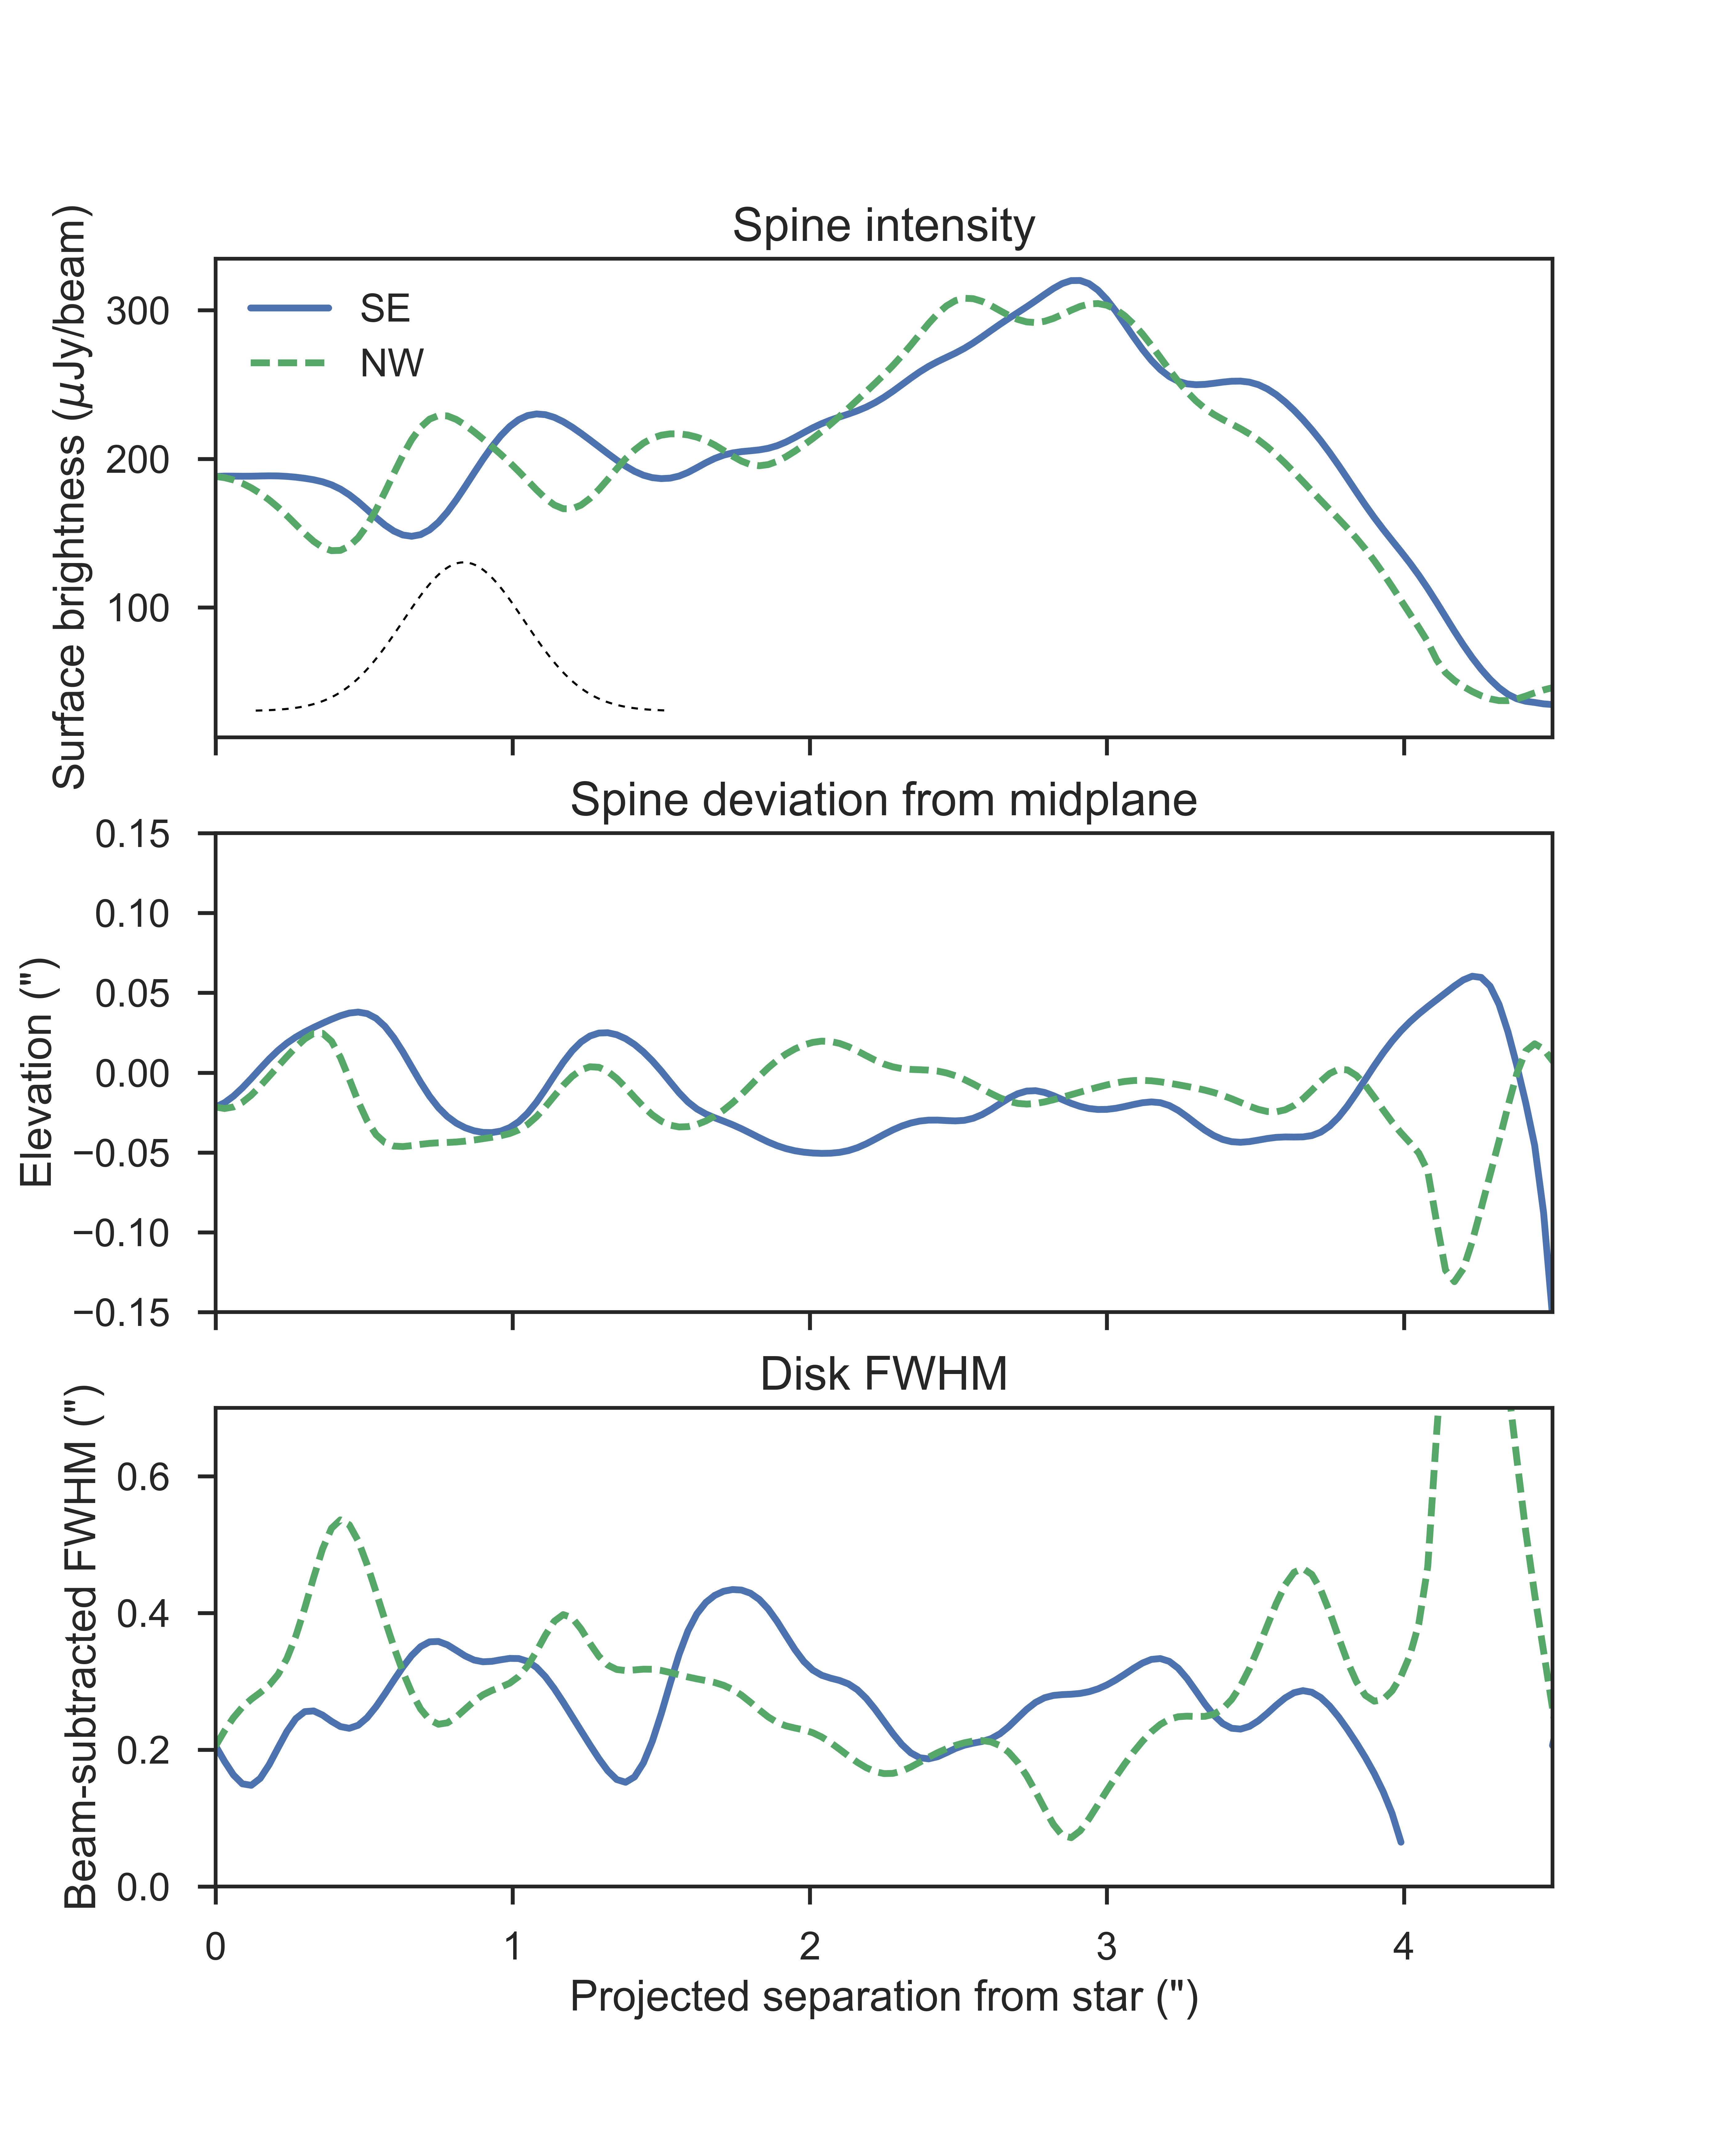
\includegraphics[width=.75\linewidth]{figures/3_boccaletti_plots}
  \caption{
  Image-domain analysis of AU Mic's radial structure. 
  At each radial location along the disk midplane, a 1-D Gaussian was fit to the vertical surface brightness profile at that location.
  From top to bottom, the three plots show the amplitude, centroid and width of the Gaussian fit as a function of angular separation from the star. 
  The Gaussian traced by the dotted line in the upper pane shows the width of the  synthesized beam in the radial direction.
  In the bottom pane, the broadening effects of the synthesized beam in the vertical direction have been removed; the fact that the image-domain vertical height of the disk is in excess of the beam contribution implies that our data spatially resolve the vertical structure of the disk.} 
  \label{fig: boccaletti}
\end{figure}


\chapter{Analysis}
To more rigorously analyze geometric structure of the disk and the emissive properties of the constituent dust, we model the ALMA observations directly in the visibility domain.
First, a model sky image is created by a ray-tracing code from a 2-D density and temperature grid. 
The spatial resolution of the model image is \SI{0.3}{au} per pixel, i.e. \SI{10}{\percent} of the spatial scale sampled by the longest baseline in the data.
The model image is then sampled at the same spatial frequencies as the ALMA data and Fourier transformed into the visibility domain with the \texttt{MIRIAD} task \texttt{uvmodel}; this allows the model to be compared directly to the interferometric data, for which the uncertainties are better understood.
A $\chi^2$ metric is used to asses the quality of the fit.

\section{Modeling Formalism}
We assume the disk to be optically thing and devoid of significant levels of dust.
\begin{itemize}
  \item Evan talks about model here?
\end{itemize}


\section{MCMC Fitting}
We explore the parameter space of the model using a Markov Chain Monte Carlo (MCMC) routine. Specifically, we use the affine-invariant formulation described by \cite{goodmanweare10} and implemented in Python as \texttt{emcee} \citep{foreman-mackey13}.  MCMC methods sample the full breadth of the parameter space associated with a specific model, allowing the posterior probability function of each parameter to be estimated. As such, the process not only identifies regions of high probability in parameter space, but uncertainties and degeneracies between parameters can be determined by examining the correlations the posteriors of each parameter.

\begin{table}
  \caption{MCMC}
  \label{tab: params}
  \begin{tabular}{lr}
  \toprule
    \multirow{2}{*}{Parameter} &
    \multicolumn{2}{|c|}{\bfseries Implemented in}\\ \cline{3-4} \\
  \midrule
    $\log$ Disk Mass (\si{\Msun}) & \\
    SB Law &  \\
    Scale Factor &  \\
    $r_{in}$ (\si{au}) &  \\
    $r_{out}$ (\si{au}) &  \\
    $i$ (\si{\degree}) &  \\
    PA  (\si{\degree}) &  \\
    March $F_*$ (\si{\micro Jy}) &  \\
    August $F_*$ (\si{\micro Jy}) &  \\
    June $F_*$ (\si{\micro Jy}) &   \\
    lnprob \\
  \bottomrule
  \end{tabular}
\end{table}

\begin{enumerate}
  \item Describe model \& model pipeline
  \item weighting goes here?
\end{enumerate}


%===============================================================================
% APPENDIX
% \appendix 
%===============================================================================
% BIBLIOGRAPHY:
\bibliography{thesis_bib}
%===============================================================================
\end{document} 
